% Options for packages loaded elsewhere
\PassOptionsToPackage{unicode}{hyperref}
\PassOptionsToPackage{hyphens}{url}
%
\documentclass[
]{book}
\usepackage{amsmath,amssymb}
\usepackage{lmodern}
\usepackage{iftex}
\ifPDFTeX
  \usepackage[T1]{fontenc}
  \usepackage[utf8]{inputenc}
  \usepackage{textcomp} % provide euro and other symbols
\else % if luatex or xetex
  \usepackage{unicode-math}
  \defaultfontfeatures{Scale=MatchLowercase}
  \defaultfontfeatures[\rmfamily]{Ligatures=TeX,Scale=1}
\fi
% Use upquote if available, for straight quotes in verbatim environments
\IfFileExists{upquote.sty}{\usepackage{upquote}}{}
\IfFileExists{microtype.sty}{% use microtype if available
  \usepackage[]{microtype}
  \UseMicrotypeSet[protrusion]{basicmath} % disable protrusion for tt fonts
}{}
\makeatletter
\@ifundefined{KOMAClassName}{% if non-KOMA class
  \IfFileExists{parskip.sty}{%
    \usepackage{parskip}
  }{% else
    \setlength{\parindent}{0pt}
    \setlength{\parskip}{6pt plus 2pt minus 1pt}}
}{% if KOMA class
  \KOMAoptions{parskip=half}}
\makeatother
\usepackage{xcolor}
\usepackage{color}
\usepackage{fancyvrb}
\newcommand{\VerbBar}{|}
\newcommand{\VERB}{\Verb[commandchars=\\\{\}]}
\DefineVerbatimEnvironment{Highlighting}{Verbatim}{commandchars=\\\{\}}
% Add ',fontsize=\small' for more characters per line
\usepackage{framed}
\definecolor{shadecolor}{RGB}{248,248,248}
\newenvironment{Shaded}{\begin{snugshade}}{\end{snugshade}}
\newcommand{\AlertTok}[1]{\textcolor[rgb]{0.94,0.16,0.16}{#1}}
\newcommand{\AnnotationTok}[1]{\textcolor[rgb]{0.56,0.35,0.01}{\textbf{\textit{#1}}}}
\newcommand{\AttributeTok}[1]{\textcolor[rgb]{0.77,0.63,0.00}{#1}}
\newcommand{\BaseNTok}[1]{\textcolor[rgb]{0.00,0.00,0.81}{#1}}
\newcommand{\BuiltInTok}[1]{#1}
\newcommand{\CharTok}[1]{\textcolor[rgb]{0.31,0.60,0.02}{#1}}
\newcommand{\CommentTok}[1]{\textcolor[rgb]{0.56,0.35,0.01}{\textit{#1}}}
\newcommand{\CommentVarTok}[1]{\textcolor[rgb]{0.56,0.35,0.01}{\textbf{\textit{#1}}}}
\newcommand{\ConstantTok}[1]{\textcolor[rgb]{0.00,0.00,0.00}{#1}}
\newcommand{\ControlFlowTok}[1]{\textcolor[rgb]{0.13,0.29,0.53}{\textbf{#1}}}
\newcommand{\DataTypeTok}[1]{\textcolor[rgb]{0.13,0.29,0.53}{#1}}
\newcommand{\DecValTok}[1]{\textcolor[rgb]{0.00,0.00,0.81}{#1}}
\newcommand{\DocumentationTok}[1]{\textcolor[rgb]{0.56,0.35,0.01}{\textbf{\textit{#1}}}}
\newcommand{\ErrorTok}[1]{\textcolor[rgb]{0.64,0.00,0.00}{\textbf{#1}}}
\newcommand{\ExtensionTok}[1]{#1}
\newcommand{\FloatTok}[1]{\textcolor[rgb]{0.00,0.00,0.81}{#1}}
\newcommand{\FunctionTok}[1]{\textcolor[rgb]{0.00,0.00,0.00}{#1}}
\newcommand{\ImportTok}[1]{#1}
\newcommand{\InformationTok}[1]{\textcolor[rgb]{0.56,0.35,0.01}{\textbf{\textit{#1}}}}
\newcommand{\KeywordTok}[1]{\textcolor[rgb]{0.13,0.29,0.53}{\textbf{#1}}}
\newcommand{\NormalTok}[1]{#1}
\newcommand{\OperatorTok}[1]{\textcolor[rgb]{0.81,0.36,0.00}{\textbf{#1}}}
\newcommand{\OtherTok}[1]{\textcolor[rgb]{0.56,0.35,0.01}{#1}}
\newcommand{\PreprocessorTok}[1]{\textcolor[rgb]{0.56,0.35,0.01}{\textit{#1}}}
\newcommand{\RegionMarkerTok}[1]{#1}
\newcommand{\SpecialCharTok}[1]{\textcolor[rgb]{0.00,0.00,0.00}{#1}}
\newcommand{\SpecialStringTok}[1]{\textcolor[rgb]{0.31,0.60,0.02}{#1}}
\newcommand{\StringTok}[1]{\textcolor[rgb]{0.31,0.60,0.02}{#1}}
\newcommand{\VariableTok}[1]{\textcolor[rgb]{0.00,0.00,0.00}{#1}}
\newcommand{\VerbatimStringTok}[1]{\textcolor[rgb]{0.31,0.60,0.02}{#1}}
\newcommand{\WarningTok}[1]{\textcolor[rgb]{0.56,0.35,0.01}{\textbf{\textit{#1}}}}
\usepackage{longtable,booktabs,array}
\usepackage{calc} % for calculating minipage widths
% Correct order of tables after \paragraph or \subparagraph
\usepackage{etoolbox}
\makeatletter
\patchcmd\longtable{\par}{\if@noskipsec\mbox{}\fi\par}{}{}
\makeatother
% Allow footnotes in longtable head/foot
\IfFileExists{footnotehyper.sty}{\usepackage{footnotehyper}}{\usepackage{footnote}}
\makesavenoteenv{longtable}
\usepackage{graphicx}
\makeatletter
\def\maxwidth{\ifdim\Gin@nat@width>\linewidth\linewidth\else\Gin@nat@width\fi}
\def\maxheight{\ifdim\Gin@nat@height>\textheight\textheight\else\Gin@nat@height\fi}
\makeatother
% Scale images if necessary, so that they will not overflow the page
% margins by default, and it is still possible to overwrite the defaults
% using explicit options in \includegraphics[width, height, ...]{}
\setkeys{Gin}{width=\maxwidth,height=\maxheight,keepaspectratio}
% Set default figure placement to htbp
\makeatletter
\def\fps@figure{htbp}
\makeatother
\setlength{\emergencystretch}{3em} % prevent overfull lines
\providecommand{\tightlist}{%
  \setlength{\itemsep}{0pt}\setlength{\parskip}{0pt}}
\setcounter{secnumdepth}{5}
\usepackage{booktabs}
\usepackage{amsthm}
\makeatletter
\def\thm@space@setup{%
  \thm@preskip=8pt plus 2pt minus 4pt
  \thm@postskip=\thm@preskip
}
\makeatother
\usepackage{booktabs}
\usepackage{longtable}
\usepackage{array}
\usepackage{multirow}
\usepackage{wrapfig}
\usepackage{float}
\usepackage{colortbl}
\usepackage{pdflscape}
\usepackage{tabu}
\usepackage{threeparttable}
\usepackage{threeparttablex}
\usepackage[normalem]{ulem}
\usepackage{makecell}
\usepackage{xcolor}
\ifLuaTeX
  \usepackage{selnolig}  % disable illegal ligatures
\fi
\usepackage[]{natbib}
\bibliographystyle{apalike}
\IfFileExists{bookmark.sty}{\usepackage{bookmark}}{\usepackage{hyperref}}
\IfFileExists{xurl.sty}{\usepackage{xurl}}{} % add URL line breaks if available
\urlstyle{same} % disable monospaced font for URLs
\hypersetup{
  pdftitle={Center for Conservation Biology \textbar{} UC Riverside},
  pdfauthor={Lynn Sweet \textbar{} Principal Investigator, Assistant Research Ecologist; Julia Parish \textbar{} Data Science Intern},
  hidelinks,
  pdfcreator={LaTeX via pandoc}}

\title{Center for Conservation Biology \textbar{} UC Riverside}
\usepackage{etoolbox}
\makeatletter
\providecommand{\subtitle}[1]{% add subtitle to \maketitle
  \apptocmd{\@title}{\par {\large #1 \par}}{}{}
}
\makeatother
\subtitle{Installation Guide}
\author{Lynn Sweet \textbar{} Principal Investigator, Assistant Research Ecologist \and Julia Parish \textbar{} Data Science Intern}
\date{2022-08-02}

\begin{document}
\maketitle

{
\setcounter{tocdepth}{1}
\tableofcontents
}
\hypertarget{informational-resource-for-software-and-application-installation-utilized-by-ccb-faculty-staff}{%
\chapter*{Informational Resource for Software and Application Installation Utilized by CCB Faculty \& Staff}\label{informational-resource-for-software-and-application-installation-utilized-by-ccb-faculty-staff}}
\addcontentsline{toc}{chapter}{Informational Resource for Software and Application Installation Utilized by CCB Faculty \& Staff}

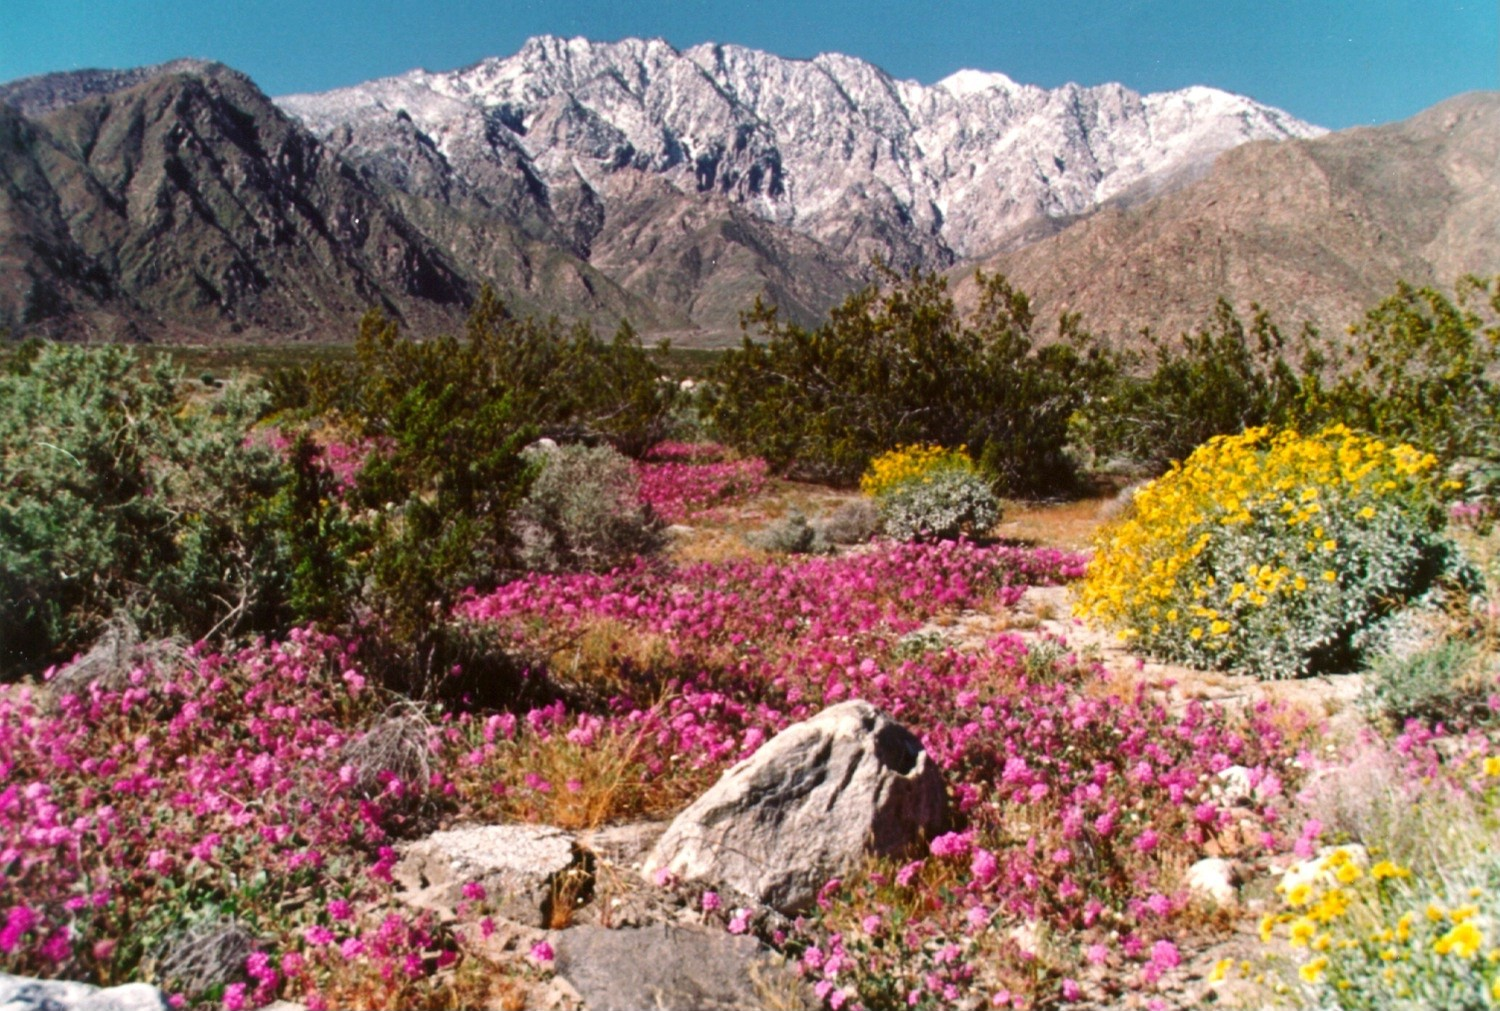
\includegraphics[width=20.83in]{images/cvmc_billhavert}

Chino Canyon Wildflowers, Coachella Valley, California.
\textbf{Image Credit:} Coachella Valley Mountains Conservancy: \emph{Bill Havert}

\begin{center}
\includegraphics[width=12.85in]{images/ucrccb} \end{center}

\hypertarget{intro}{%
\chapter{Introduction}\label{intro}}

This is an installation and account set up reference guide for the Center for Conservation Biology team. Team members may contribute to this reference file as we expand the tools utlizied during research efforts.

\hypertarget{computer-requirements}{%
\section{Computer requirements}\label{computer-requirements}}

Work computers (laptop or desktop) operating systems should either be Windows or macOS. Please note that Windows based machine it required to run ESRI ArcDesktop and ArcPro software. Both Windows and macOS may utilize ESRI ArcOnline tools.

For \textbf{Mac} users, update macOS to the newest supported version. Navigate to System Preferences --\textgreater{} Software Update.

For \textbf{PC} users, ensure you have Windows 10 or 11 installed. If not, request a Windows key from UCR IT at \href{https://ucrsupport.service-now.com/ucr_portal?id=ucr_home}{UC Riverside ServiceLink}

\hypertarget{software}{%
\section{Software}\label{software}}

Software covered in this reference guide includes:

\begin{itemize}
\tightlist
\item
  git
\item
  GitHub
\item
  Google Apps
\item
  R
\item
  RStudio

  \begin{itemize}
  \tightlist
  \item
    Quarto
  \item
    Bookdown
  \end{itemize}
\item
  Slack
\item
  Trello

  \begin{itemize}
  \tightlist
  \item
    Trello 4 Slack
  \end{itemize}
\item
  Zotero
\end{itemize}

\begin{center}\rule{0.5\linewidth}{0.5pt}\end{center}

Thank you to UC Santa Barbara's Bren School of Environmental Science \& Management and National Center for Ecological Analysis and Synthesis (NCEAS) staff for providing many of the resources listed in this reference guide. Information was made available on the \href{https://github.com/UCSB-MEDS}{UCSB-MEDS GitHub page}.

\hypertarget{r}{%
\chapter{R and RStudio Installation}\label{r}}

\hypertarget{install-or-update-r}{%
\section{Install or Update R}\label{install-or-update-r}}

\textbf{R} is a programming language and environment used for statistical computing and grahics. For more information, please visit \href{https://www.r-project.org/about.html}{What is R}.

To install R, visit \href{https://cloud.r-project.org/}{cloud.r-project.org} to download the most recent version for your operating system.

\hypertarget{install-or-update-r-studio}{%
\section{Install or Update R Studio}\label{install-or-update-r-studio}}

RStudio is a software (considered an Integrated Development Environment, or IDE) that provides R programmers with an easy-to-use interface for coding in R.

\textbf{Note:} RStudio will not work without R installed, and you won't particularly enjoy using R without having RStudio installed. Be sure to install both!

\begin{itemize}
\item
  \textbf{New install:} To install RStudio, visit \href{https://www.rstudio.com/products/rstudio/}{rstudio.com/products/rstudio/}. Download the free (``Open Source Edition'') Desktop version for your operating system.
\item
  \textbf{Update:} If you already have RStudio and need to update: Open RStudio, and under `Help' in the top menu, choose `Check for updates.' If you have the most recent release, it will return `No update available. You are running the most recent version of RStudio.' Otherwise, you should follow the instructions to install an updated version.
\end{itemize}

Open RStudio (logo you'll click on shown below). \textbf{If you are prompted to install Command Line Tools, do it.}

\begin{center}
\includegraphics[width=4.97in]{images/rstudio} \end{center}

\textbf{Mac Users}

There may be a need to install command line tools and \href{https://www.xquartz.org/}{XQuartz}:

\begin{itemize}
\item
  To install command line tools (if you're not automatically prompted), run in the Terminal tab in RStudio: \texttt{xcode-select\ -\/-install}
\item
  Visit \href{https://www.xquartz.org/}{xquartz.org} to download \& install XQuartz.
\end{itemize}

\hypertarget{install-quarto}{%
\section{Install Quarto}\label{install-quarto}}

\emph{This is an optional tool within R Studio that is extremely powerful, but it is not required.}

Quarto is a scientific publishing tool built on Pandoc that allows R, Python, Julia, and ObservableJS users to create dynamic documents, websites, books and more.

As of \emph{July 2022}, Quarto comes pre-installed in R Studio (v2022.07). If you haven't updated your R Studio IDE (and concerned about doing so), you can install Quarto separately.

\begin{itemize}
\item
  Download Quarto \href{https://quarto.org/docs/get-started/}{here} and install
\item
  To use Quarto through the RStudio IDE, be sure to have at least version v2022.02 installed (see directions in step 2, above)
\end{itemize}

Learn more about Quarto \href{https://quarto.org/docs/get-started/hello/rstudio.html}{here}.

\hypertarget{learn-how-to-use-r-rstudio}{%
\section{Learn How to Use R \& RStudio}\label{learn-how-to-use-r-rstudio}}

There are a lot of resources out there to help you learn how to use R and the RStudio IDE (YouTube, Googling, \href{https://stackoverflow.com/}{StackOverflow}, etc\ldots). This is a short list of primary resources for you to reference. It is highly recommended to join R community Slack channels, R User community groups (such as \href{https://rladies.org/}{R-Ladies}), and UC Riverside Data Science clubs!

\begin{itemize}
\tightlist
\item
  \href{https://acmucr.org/index.html}{ACM at UCR} - UC Riverside community dedicated to technical, professional, and personal development in the context of computer science.
\item
  \href{https://r4ds.had.co.nz/}{R for Data Science}
\item
  \href{https://bookdown.org/yihui/rmarkdown-cookbook/}{R Markdown Cookbook}
\item
  \href{http://www.cookbook-r.com/}{Cookbook for R}
\item
  \href{https://adv-r.hadley.nz/}{Advanced R}
\item
  \href{https://www.rstudio.com/resources/books/}{R Studio (posit) Book Catalog}
\item
  \href{https://www.rfordatasci.com/}{R for Data Science Online Learning Community}
\item
  \href{https://ropensci.org/}{R OpenSci}
\item
  \href{https://rstudio.cloud/learn/primers}{RStudio Cloud} - interactive tutorials to learn data science basics.
\item
  \href{https://www.rstudio.com/resources/cheatsheets/}{R Studio Cheatsheets} - invaluable tool to learn how to use various R packages.
\item
  \href{https://swirlstats.com/}{Swirl} - R package that is a built in tutorial.
\end{itemize}

\hypertarget{bookdown}{%
\chapter{Bookdown Guide}\label{bookdown}}

The first step to edit and add to this bookdown is to install the \textbf{bookdown} package from CRAN or Github. In the RStudio console, run the following:

\begin{Shaded}
\begin{Highlighting}[]
\FunctionTok{install.packages}\NormalTok{(}\StringTok{"bookdown"}\NormalTok{)}
\CommentTok{\# or the development version}
\CommentTok{\# devtools::install\_github(\textquotesingle{}rstudio/bookdown\textquotesingle{})}
\end{Highlighting}
\end{Shaded}

\hypertarget{primary-reference-resources}{%
\section{Primary Reference Resources}\label{primary-reference-resources}}

Here is a list of resources to learn how to use and edit in bookdown

\begin{itemize}
\tightlist
\item
  \href{https://bookdown.org/}{Bookdown Package Documentation}
\item
  \href{https://bookdown.org/yihui/bookdown/}{Authoring Books with R Markdown}
\item
  \href{https://bookdown.org/yihui/rmarkdown-cookbook/}{R Markdown Cookbook}
\item
  \href{https://bookdown.org/yihui/rmarkdown/}{R Markdown: The Definitive Guide}
\end{itemize}

\begin{center}\rule{0.5\linewidth}{0.5pt}\end{center}

\textbf{The following information is directly taken from the \emph{bookdown} package} \citep{R-bookdown}.

\hypertarget{formatting}{%
\section{Formatting}\label{formatting}}

You can use anything that Pandoc's Markdown supports, e.g., a math equation \(a^2 + b^2 = c^2\).

Remember each Rmd file contains one and only one chapter, and \textbf{a chapter} is defined by the first-level heading \texttt{\#}.

You can label chapter and section titles using \texttt{\{\#label\}} after them, e.g., we can reference Chapter \ref{intro}. If you do not manually label them, there will be automatic labels anyway, e.g., Chapter \ref{methods}.

Figures and tables with captions will be placed in \texttt{figure} and \texttt{table} environments, respectively.

\begin{figure}

{\centering 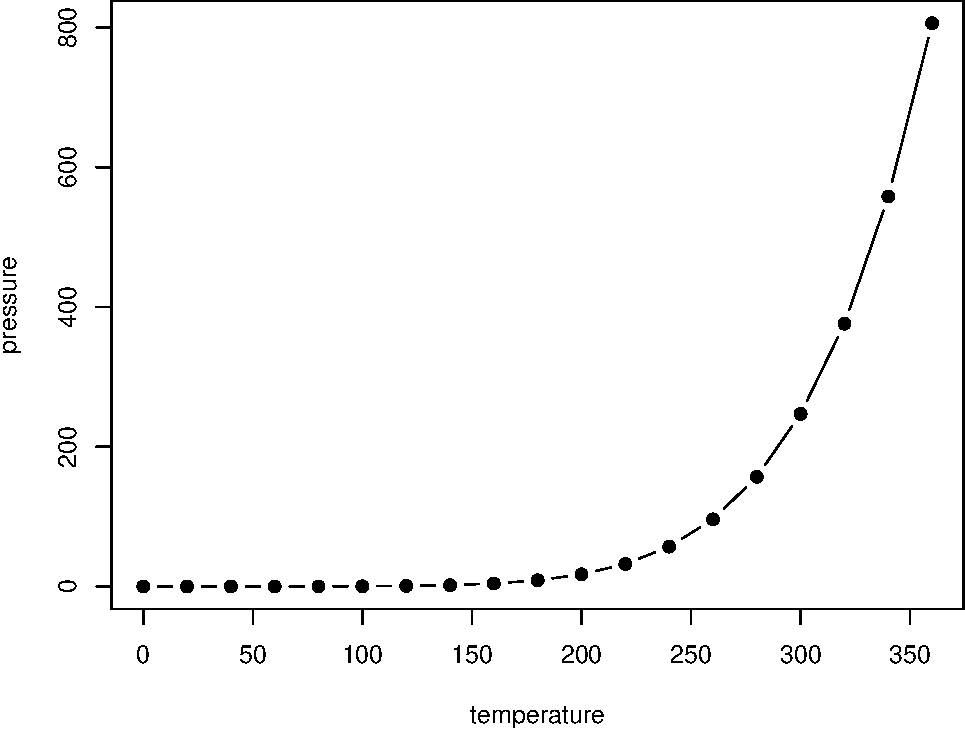
\includegraphics[width=0.8\linewidth]{bookdown-demo_files/figure-latex/nice-fig-1} 

}

\caption{Here is a nice figure!}\label{fig:nice-fig}
\end{figure}

Reference a figure by its code chunk label with the \texttt{fig:} prefix, e.g., see Figure \ref{fig:nice-fig}. Similarly, you can reference tables generated from \texttt{knitr::kable()}, e.g., see Table \ref{tab:nice-tab}.

\begin{table}

\caption{\label{tab:nice-tab}Here is a nice table!}
\centering
\begin{tabular}[t]{rrrrl}
\toprule
Sepal.Length & Sepal.Width & Petal.Length & Petal.Width & Species\\
\midrule
5.1 & 3.5 & 1.4 & 0.2 & setosa\\
4.9 & 3.0 & 1.4 & 0.2 & setosa\\
4.7 & 3.2 & 1.3 & 0.2 & setosa\\
4.6 & 3.1 & 1.5 & 0.2 & setosa\\
5.0 & 3.6 & 1.4 & 0.2 & setosa\\
\addlinespace
5.4 & 3.9 & 1.7 & 0.4 & setosa\\
4.6 & 3.4 & 1.4 & 0.3 & setosa\\
5.0 & 3.4 & 1.5 & 0.2 & setosa\\
4.4 & 2.9 & 1.4 & 0.2 & setosa\\
4.9 & 3.1 & 1.5 & 0.1 & setosa\\
\addlinespace
5.4 & 3.7 & 1.5 & 0.2 & setosa\\
4.8 & 3.4 & 1.6 & 0.2 & setosa\\
4.8 & 3.0 & 1.4 & 0.1 & setosa\\
4.3 & 3.0 & 1.1 & 0.1 & setosa\\
5.8 & 4.0 & 1.2 & 0.2 & setosa\\
\addlinespace
5.7 & 4.4 & 1.5 & 0.4 & setosa\\
5.4 & 3.9 & 1.3 & 0.4 & setosa\\
5.1 & 3.5 & 1.4 & 0.3 & setosa\\
5.7 & 3.8 & 1.7 & 0.3 & setosa\\
5.1 & 3.8 & 1.5 & 0.3 & setosa\\
\bottomrule
\end{tabular}
\end{table}

\hypertarget{citations}{%
\section{Citations}\label{citations}}

You can easily write citations using .bib files within this repository formatted using \href{http://www.bibtex.org/}{BibTEX}. For example, the \textbf{bookdown} package \citep{R-bookdown} in this reference book, which was built on top of R Markdown and \textbf{knitr} \citep{xie2015}.

\hypertarget{alt-text-for-accessibility}{%
\section{Alt Text for Accessibility}\label{alt-text-for-accessibility}}

\href{https://www.rstudio.com/blog/knitr-fig-alt/}{Use the knitr package to add alt text to graphics in R Markdown files}

\hypertarget{rendering-bookdown-to-build-publish}{%
\section{Rendering Bookdown to Build \& Publish}\label{rendering-bookdown-to-build-publish}}

In your Console, type either of these commands depending on which type of render you prefer:

\texttt{bookdown::render\_book("index.Rmd",\ "bookdown::gitbook")}
\texttt{bookdown::render\_book("index.Rmd",\ "bookdown::pdf\_book")}

To compile to PDF, you need XeLaTeX. It is recommended to install TinyTeX (which includes XeLaTeX): \url{https://yihui.name/tinytex/}.

\hypertarget{git}{%
\chapter{Git Installation \& GitHub Account}\label{git}}

\hypertarget{git-1}{%
\section{Git}\label{git-1}}

Check to see if your computer already has git:

\begin{itemize}
\tightlist
\item
  Open RStudio
\item
  In the terminal, run the following command:
\end{itemize}

\texttt{which\ git}

If \texttt{git} is already installed, the return to the above command should return a filepath (ex: \texttt{/usr/local/bin/git}).

\begin{itemize}
\tightlist
\item
  If there is no response, download and install \texttt{git} from here: \href{https://git-scm.com/downloads}{git-scm.com/downloads}. Select the default settings within the prompts \textbf{except} the default to \textbf{master} branch. This branch is being phased out, so select the option that let's you select alternative branches (ex: main).
\end{itemize}

\hypertarget{github}{%
\section{GitHub}\label{github}}

GitHub is a internet based code hosting platform for collaboration and \href{https://www.atlassian.com/git/tutorials/what-is-version-control\#:~:text=Version\%20control\%2C\%20also\%20known\%20as,to\%20source\%20code\%20over\%20time.}{version control}. GitHub lets you (and others) work together on projects.

Navigate to \href{https://github.com/}{github.com}, and create an account! Please use either your work or personal email account. You can add several emails to your account, and assign a particular email as the primary email for the account.

Review this article on choosing a GitHub username: \url{happygitwithr.com/github-acct.html}.

\hypertarget{configure-git}{%
\section{Configure Git}\label{configure-git}}

Once Git is installed and your GitHub account has been set up, Git needs to be configured on the computer. Configuring Git is required to push \& pull commits to GitHub.

\begin{itemize}
\item
  In RStudio, open the terminal.
\item
  Run the following commands separately, pressing \texttt{Enter} after each line. Replace username and email with your GitHub account username and email. Make sure to keep the quotes around the username in the code below:

  \begin{itemize}
  \tightlist
  \item
    \texttt{git\ config\ -\/-global\ user.name\ "Jane\ Doe"}
  \item
    \texttt{git\ config\ -\/-global\ user.email\ janedoe@example.com}
  \end{itemize}
\item
  Once you have entered the above command line code, check that the configuration was set correctly. In the RStudio Terminal, type the following command and hit enter:

  \begin{itemize}
  \tightlist
  \item
    \texttt{git\ config\ -\/-list\ -\/-global}
  \end{itemize}
\end{itemize}

In the terminal, it should show code similar to this in the Terminal:

\texttt{user.name=janedoe}
\texttt{user.email=janedoe@ucr.edu}
\texttt{core.excludesfile=/Users/janedoe/.gitignore}

If when installing or updating Git, the default branch was not set to \texttt{main} (it is defaulting to the old \texttt{master} branch), you can change this setting globally. In the Terminal again, enter the line below:

\texttt{git\ config\ -\/-global\ init.defaultBranch\ main}

For more information on configuring Git: \href{https://git-scm.com/book/en/v2/Getting-Started-First-Time-Git-Setup}{check out this Git reference}

\hypertarget{personal-access-token}{%
\section{Personal Access Token}\label{personal-access-token}}

Once Git has been configured to commit to your GitHub account, a \textbf{Personal Access Token (PAT)} must be created for \textbf{each computer you intend to use}. A PAT is an alternative password authentication method for Git to access GitHub accounts.

\begin{itemize}
\tightlist
\item
  In the RStudio Console, install the \href{https://usethis.r-lib.org/}{\texttt{usethis}} package in R by running the following code:
\end{itemize}

\texttt{install.packages("usethis")}

If the \texttt{usethis} package is installed correctly, at the end of the stream of text there should be a message similar to the image below:

\begin{flushleft}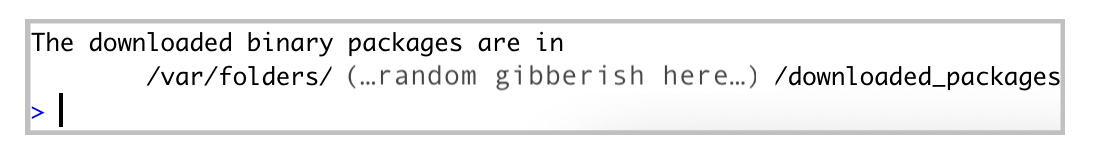
\includegraphics[width=15.39in]{images/usethis} \end{flushleft}

\begin{itemize}
\tightlist
\item
  Once the \texttt{usethis} package is installed, run the following in the RStudio Console:
\end{itemize}

\texttt{usethis::create\_github\_token()}

\begin{itemize}
\tightlist
\item
  Enter your GitHub password when prompted.
\end{itemize}

This should take you to the \textbf{Settings/Developer settings} section of your GitHub account:

\begin{flushleft}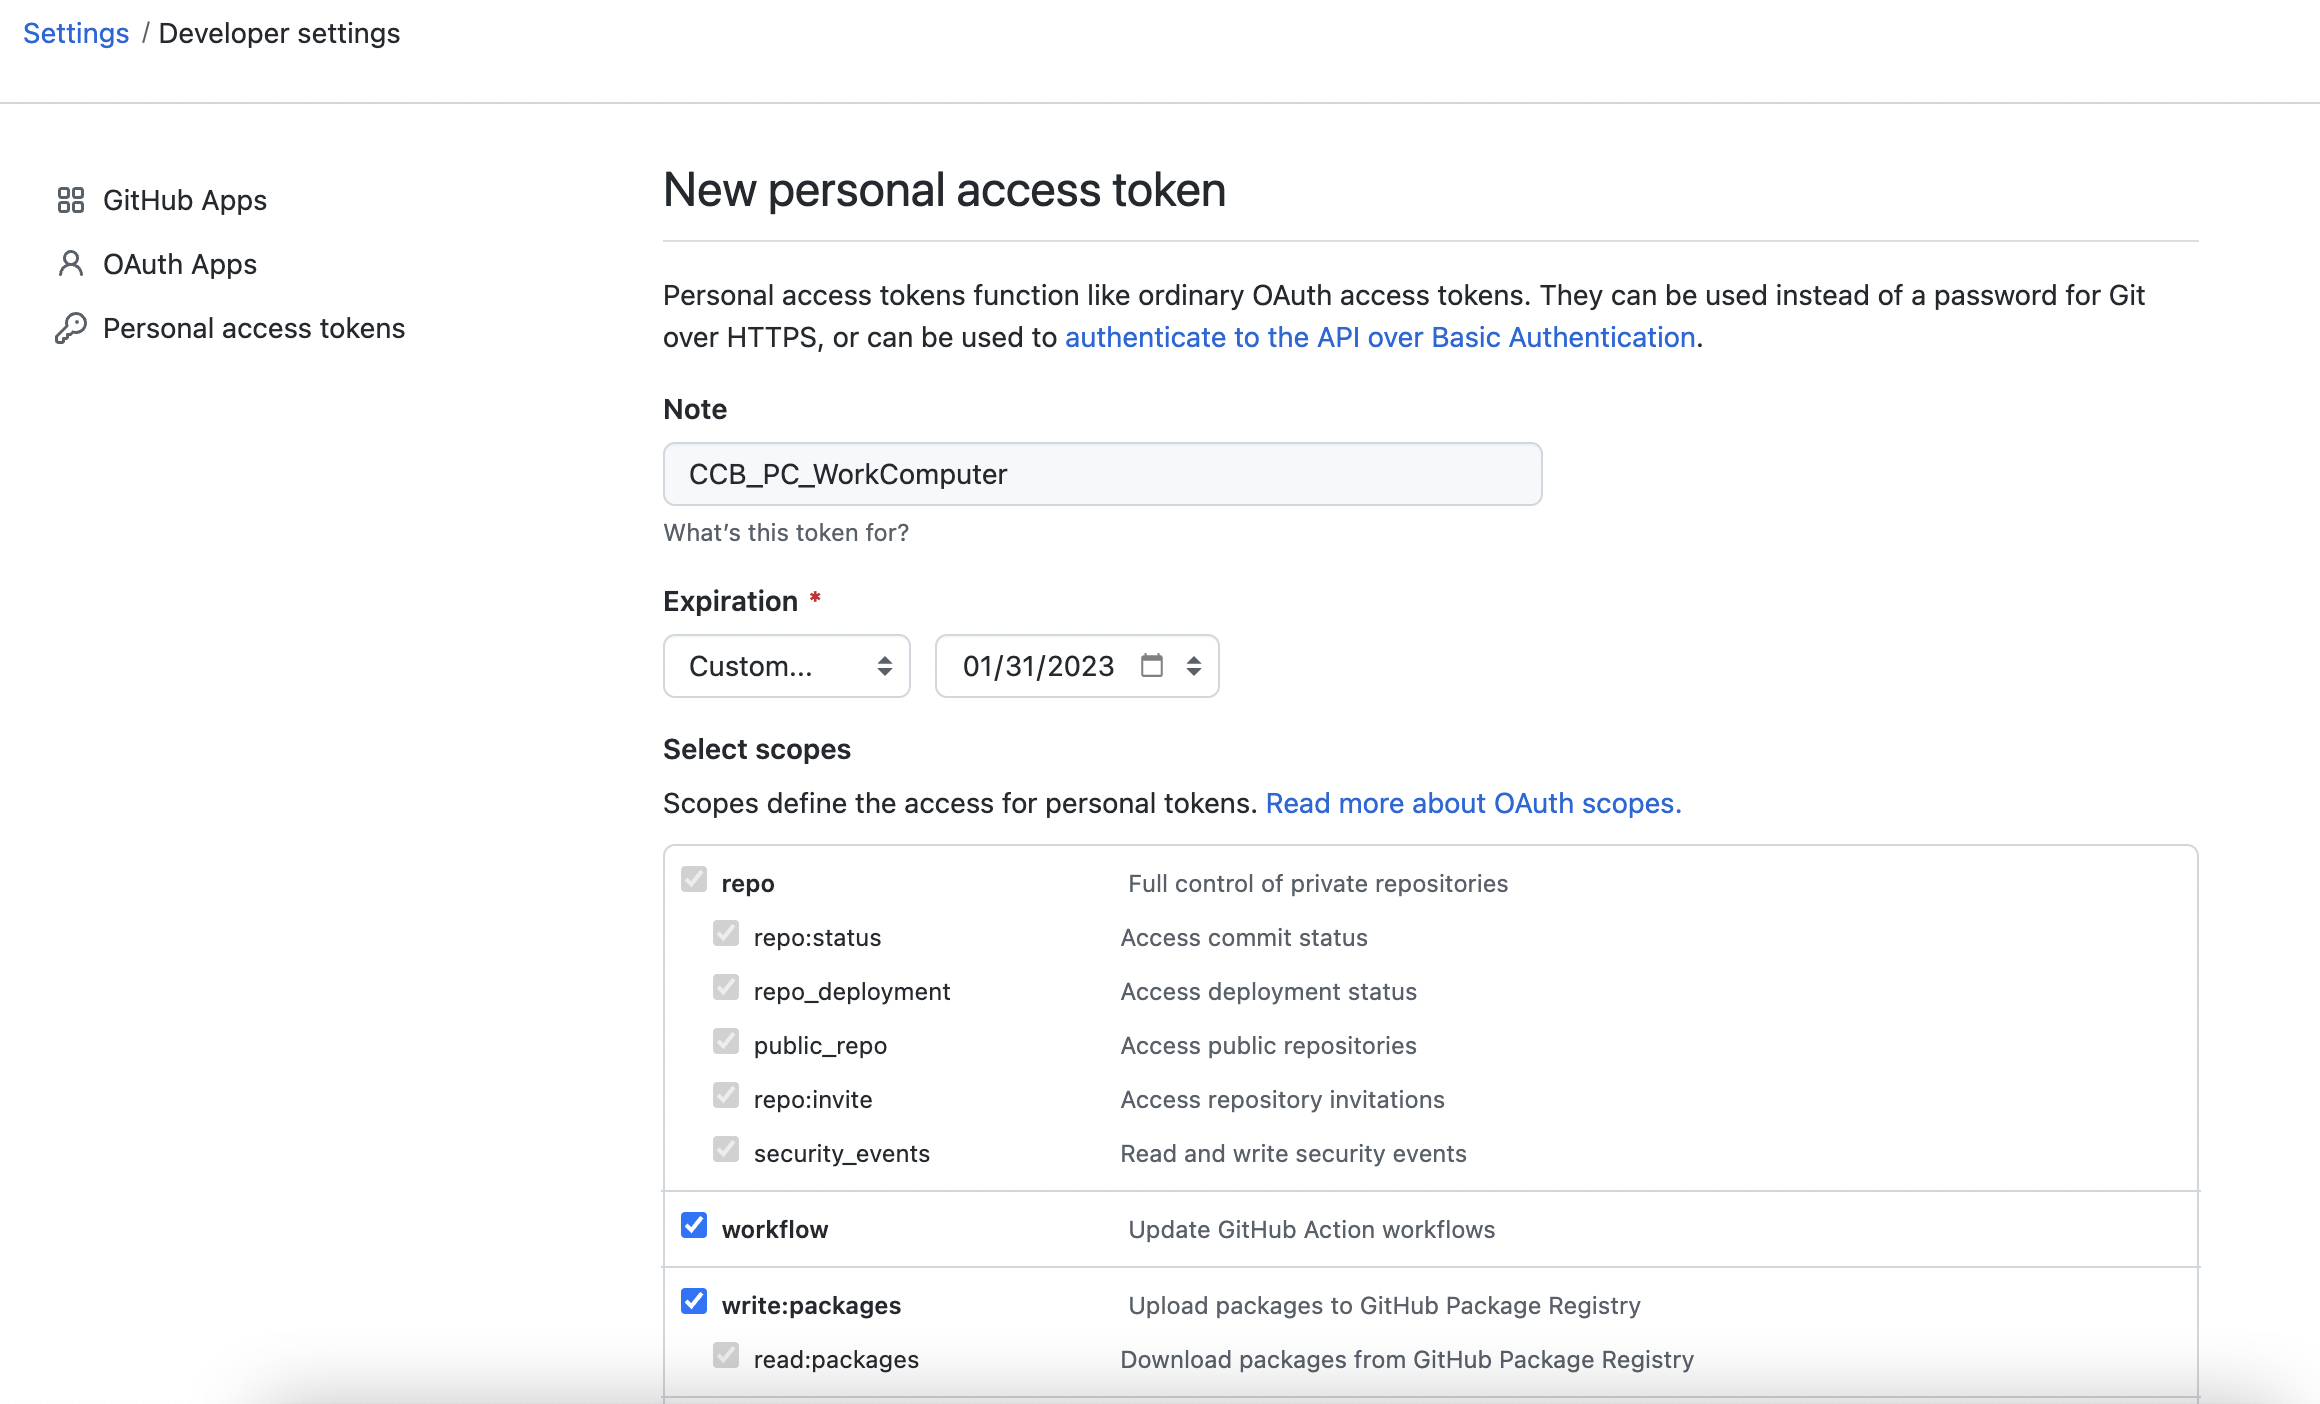
\includegraphics[width=32.22in]{images/pat} \end{flushleft}

\begin{itemize}
\item
  \textbf{Note Field}
  Change the PAT name to a meaningful reference (see image for an example). You may end up creating multiple PATs, so you want to ensure that you know which PAT is designated for each computer \textbar{} server.
\item
  \textbf{Expiration Field}
\end{itemize}

This is to select a set expiration timeframe for your PAT. Setting an expiration is highly recommended, and GitHub will send you \emph{SEVERAL} emails prior to it expiring to remind you to renew it. Use the drop down to select a set time frame (7 days to 90 days) or create a custom expiration time frame (exactly a year or particular date).

\begin{itemize}
\tightlist
\item
  \textbf{Select Scopes Field}
\end{itemize}

Define access for the Personal Access Token being generated.

It is recommended to select at least the following scopes:
- repo
- workflow
- write:packages
- notifications
- delete repo
- write:discussions
- project

To learn more about Scopes, visit \href{https://docs.github.com/en/developers/apps/building-oauth-apps/scopes-for-oauth-apps}{the GitHub Scopes for OAUth Apps page}.

\begin{itemize}
\tightlist
\item
  Once Scopes are selected, click on the green \texttt{Generate\ token} button:
\end{itemize}

\begin{center}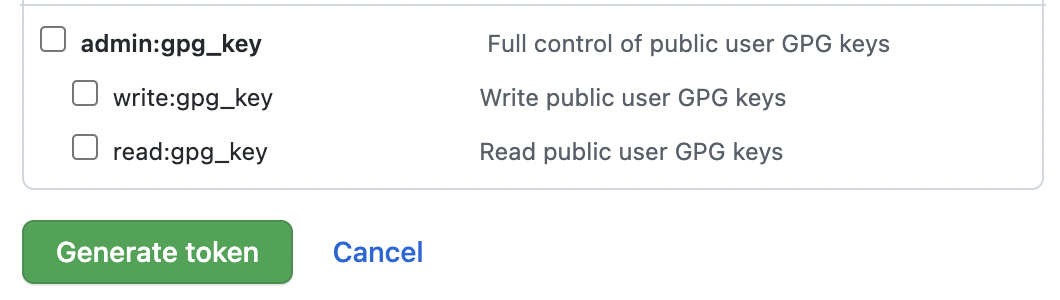
\includegraphics[width=14.72in]{images/generatepat} \end{center}

\begin{itemize}
\item
  Copy the generated PAT to your clipboard.
\item
  Paste and Save this PAT in a text file in a secure folder that will NEVER be accessed by other users or the internet. You can create a \texttt{private} folder on your personal computer to store these files.
\item
  Return to RStudio Console and run the following command:
\end{itemize}

\texttt{gitcreds::gitcreds\_set()}.

You will be prompted to paste the PAT into the console:

\begin{center}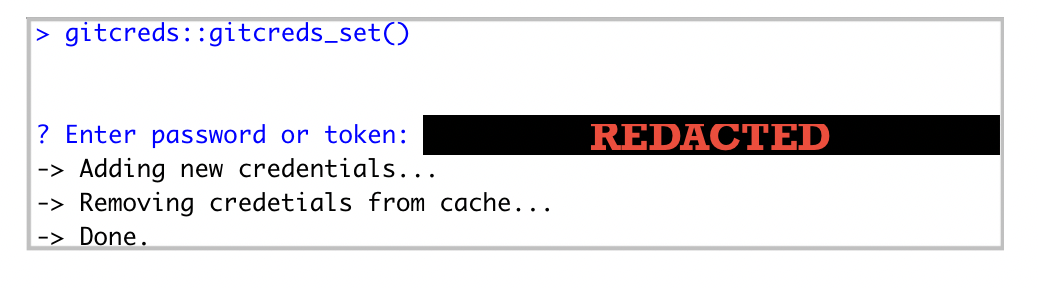
\includegraphics[width=14.42in]{images/paste_pat} \end{center}

Paste the PAT at the end of the line \texttt{Enter\ password\ or\ token:} and press enter.

\begin{itemize}
\tightlist
\item
  In the console, run:
\end{itemize}

\texttt{usethis::git\_sitrep()}

This command should return your GitHub account information (see example below).

\begin{center}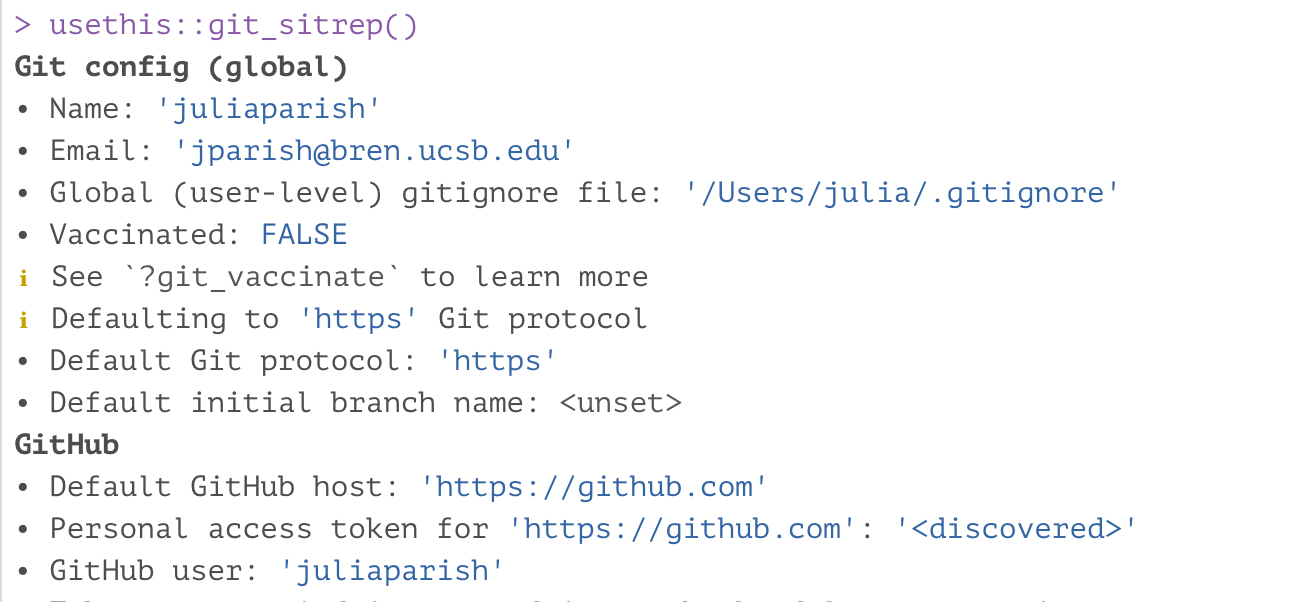
\includegraphics[width=18in]{images/gitsitrep} \end{center}

For more information on PATs, check out \href{https://docs.github.com/en/authentication/keeping-your-account-and-data-secure/creating-a-personal-access-token}{GitHub's PAT information page}.

\hypertarget{projmgmt}{%
\chapter{Project Management Tools}\label{projmgmt}}

\hypertarget{trello}{%
\section{Trello}\label{trello}}

\begin{flushleft}
\includegraphics[width=3.47in]{images/trello} \end{flushleft}

\href{https://trello.com/en}{Trello} is a project management app tool that provides teams the opportunity to create task lists, reference \& resource lists, and communicate via tagging! To connect with CCB's Trello Workspace, send a request to CCB's PI. The main board is \textbf{CCB Team Projects}.

\hypertarget{slack}{%
\section{Slack}\label{slack}}

\begin{flushleft}
\includegraphics[width=5.19in]{images/slack} \end{flushleft}

Slack is a messaging app that connects teams via channels and direct messages (DMs).
To join the CCB Slack workspace, follow \href{https://join.slack.com/t/ccbucr/shared_invite/zt-1dfpaguqs-F4CAPCI4ILMvT0JOcSpnag}{this link}.

There is a Trello app incorporated in the CCB UCR slack workspace. You can create cards in Slack for the CCB Team Projects Trello workspace. To learn how, \href{https://slack.com/help/articles/231967387-Trello-for-Slack}{follow this Slack connect tool}.

Other cool Slack workspaces to join:

\begin{itemize}
\item
  \href{https://eco-data-science.github.io/}{EcoDataScience} - an environmental data science study group that started at UC Santa Barbara, but now has an international following!
\item
  \href{https://www.rfordatasci.com}{R4DS Online Learning Community}
\item
  \href{https://www.sortee.org}{Society for Open, Reliable, and Transparent Ecology and Evolutionary Biology (SORTEE)}
\end{itemize}

\hypertarget{google-apps}{%
\section{Google Apps}\label{google-apps}}

The CCB team utilizes a number of Google applications for project management, data \& file sharing, and communicating with colleagues.

\textbf{Google Calendar:} There is a lab Google calendar, \emph{UCR CCB Palm Desert}. This calendar maintains lab mates work and leave schedules as well as any team meetings. Please make sure this calendar is shared with you once you have obtained your UCR NetId.

\textbf{Google Drive:} CCB utilizes \emph{Shared Drive} folders as a file sharing application. You must request access to the shared drive folder from the lab P.I.

\textbf{Google Sites:} There is a \href{https://sites.google.com/ucr.edu/ccbucr/home}{CCB Google Site} that is in draft form at the moment. This site may serve as an intranet or provide public facing information in the future. If you would like edit access, please submit a request to the CCB PI.

\hypertarget{zotero}{%
\section{Zotero}\label{zotero}}

The Center for Conservation Biology shares research references through Zotero software. Zotero is a citation management tool and allows groups to collect and share references easily. The Zotero browser extension makes it easy to copy citations from webpages.

To install Zotero and the extension, please follow UC Riverside's installation instructions \href{https://guides.lib.ucr.edu/c.php?g=171064}{here}. \emph{Note}: These instructions are for a \textbf{Windows} machine, but it is a similar process for Macs.

\begin{center}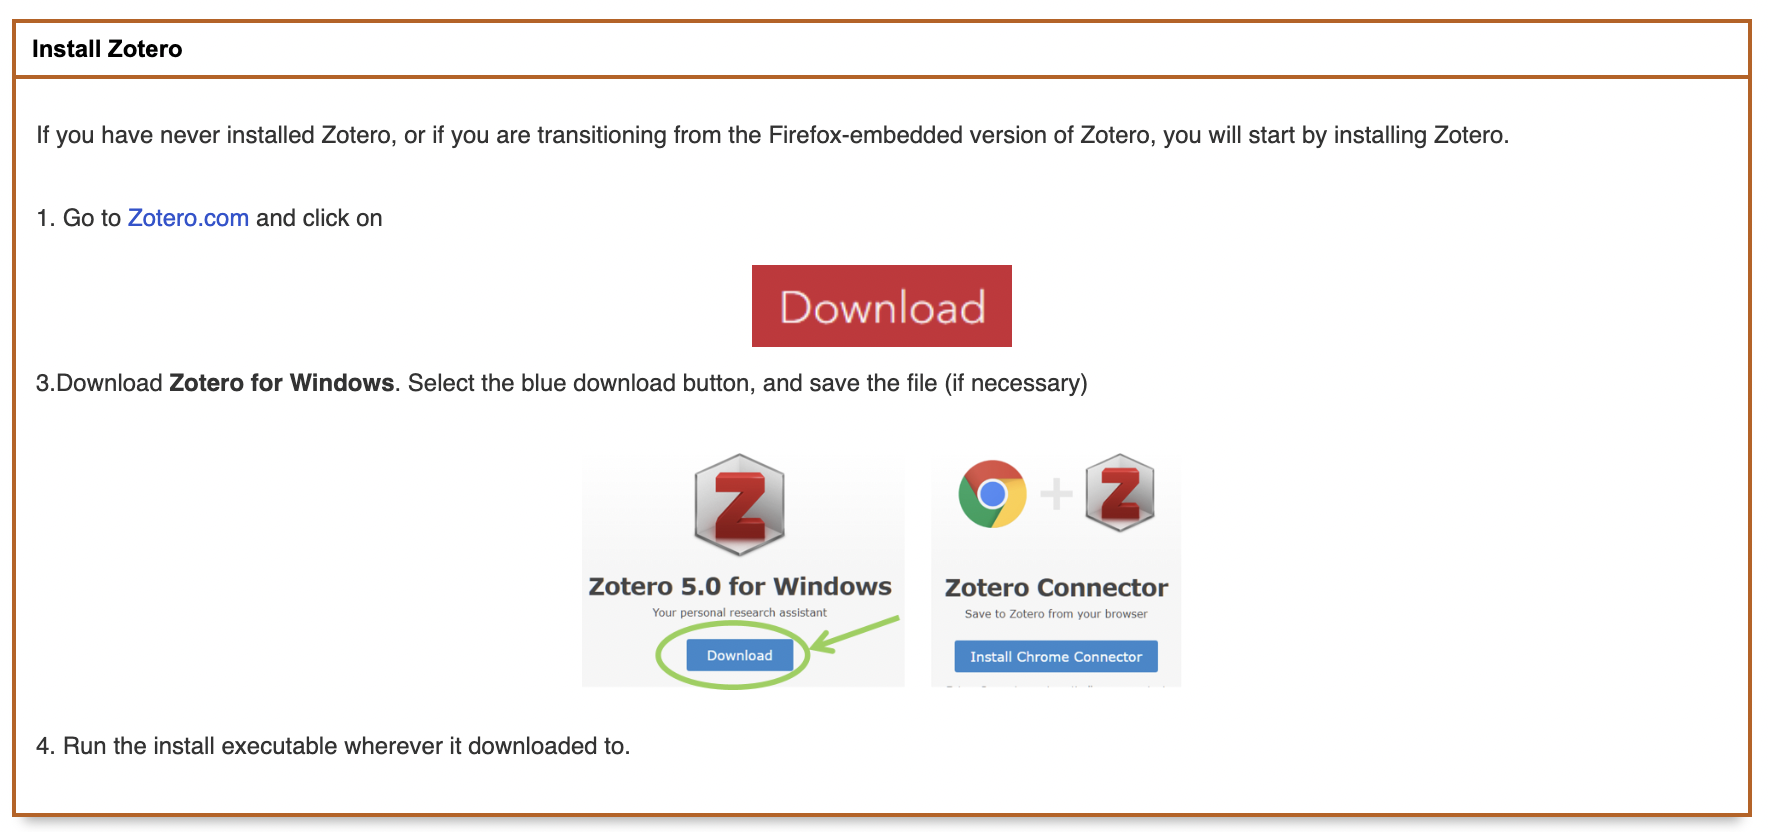
\includegraphics[width=24.56in]{images/zoteroinstall} \end{center}

\begin{center}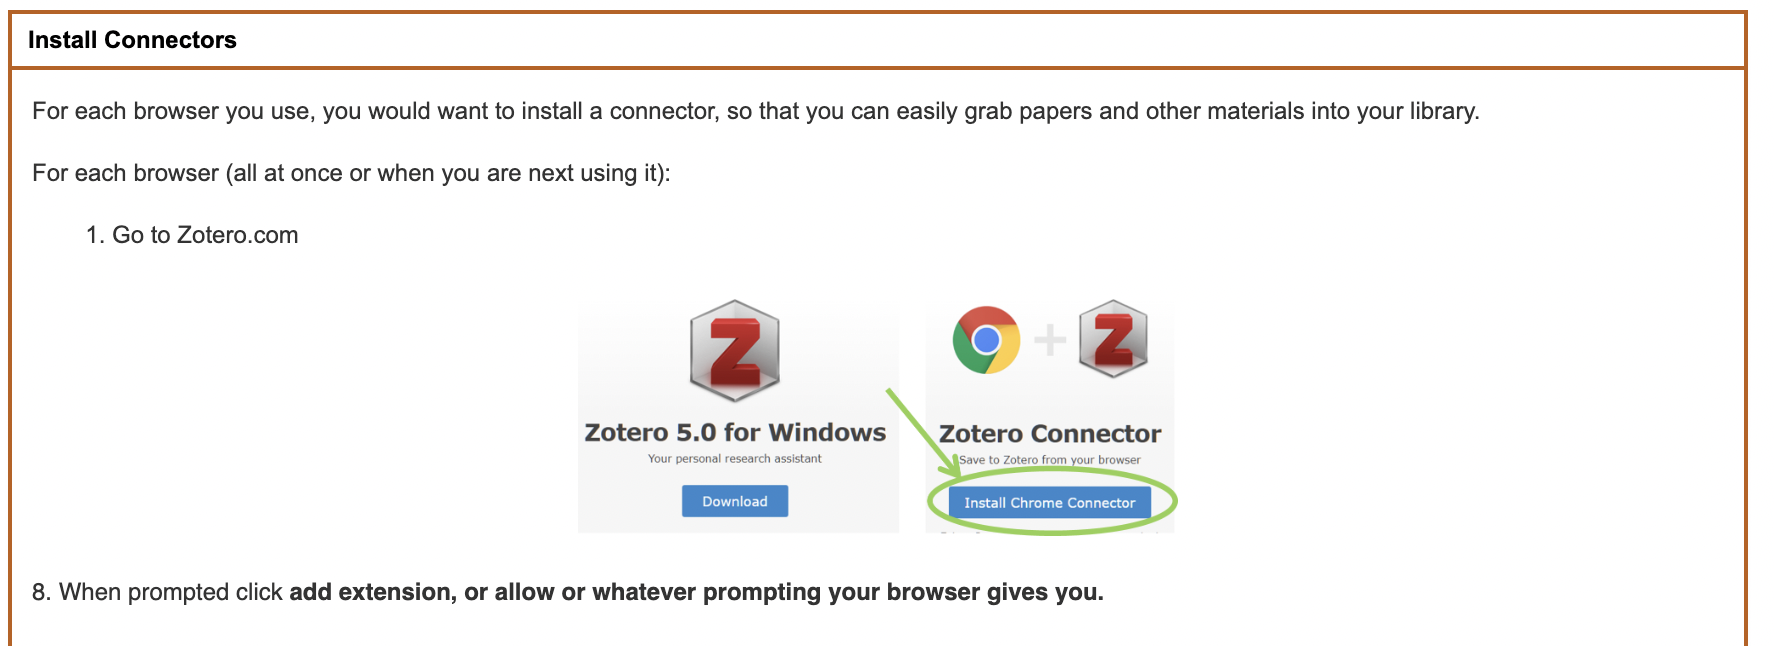
\includegraphics[width=24.64in]{images/zoteroextension} \end{center}

The next step is to create a Zotero account and enable syncing to enable extension use and to be able to join the \href{https://www.zotero.org/groups/4734848/ccbucr}{CCB Zotero Reference Group}. Make sure to use your using the UCR email address when setting up the Zotero account.

\begin{center}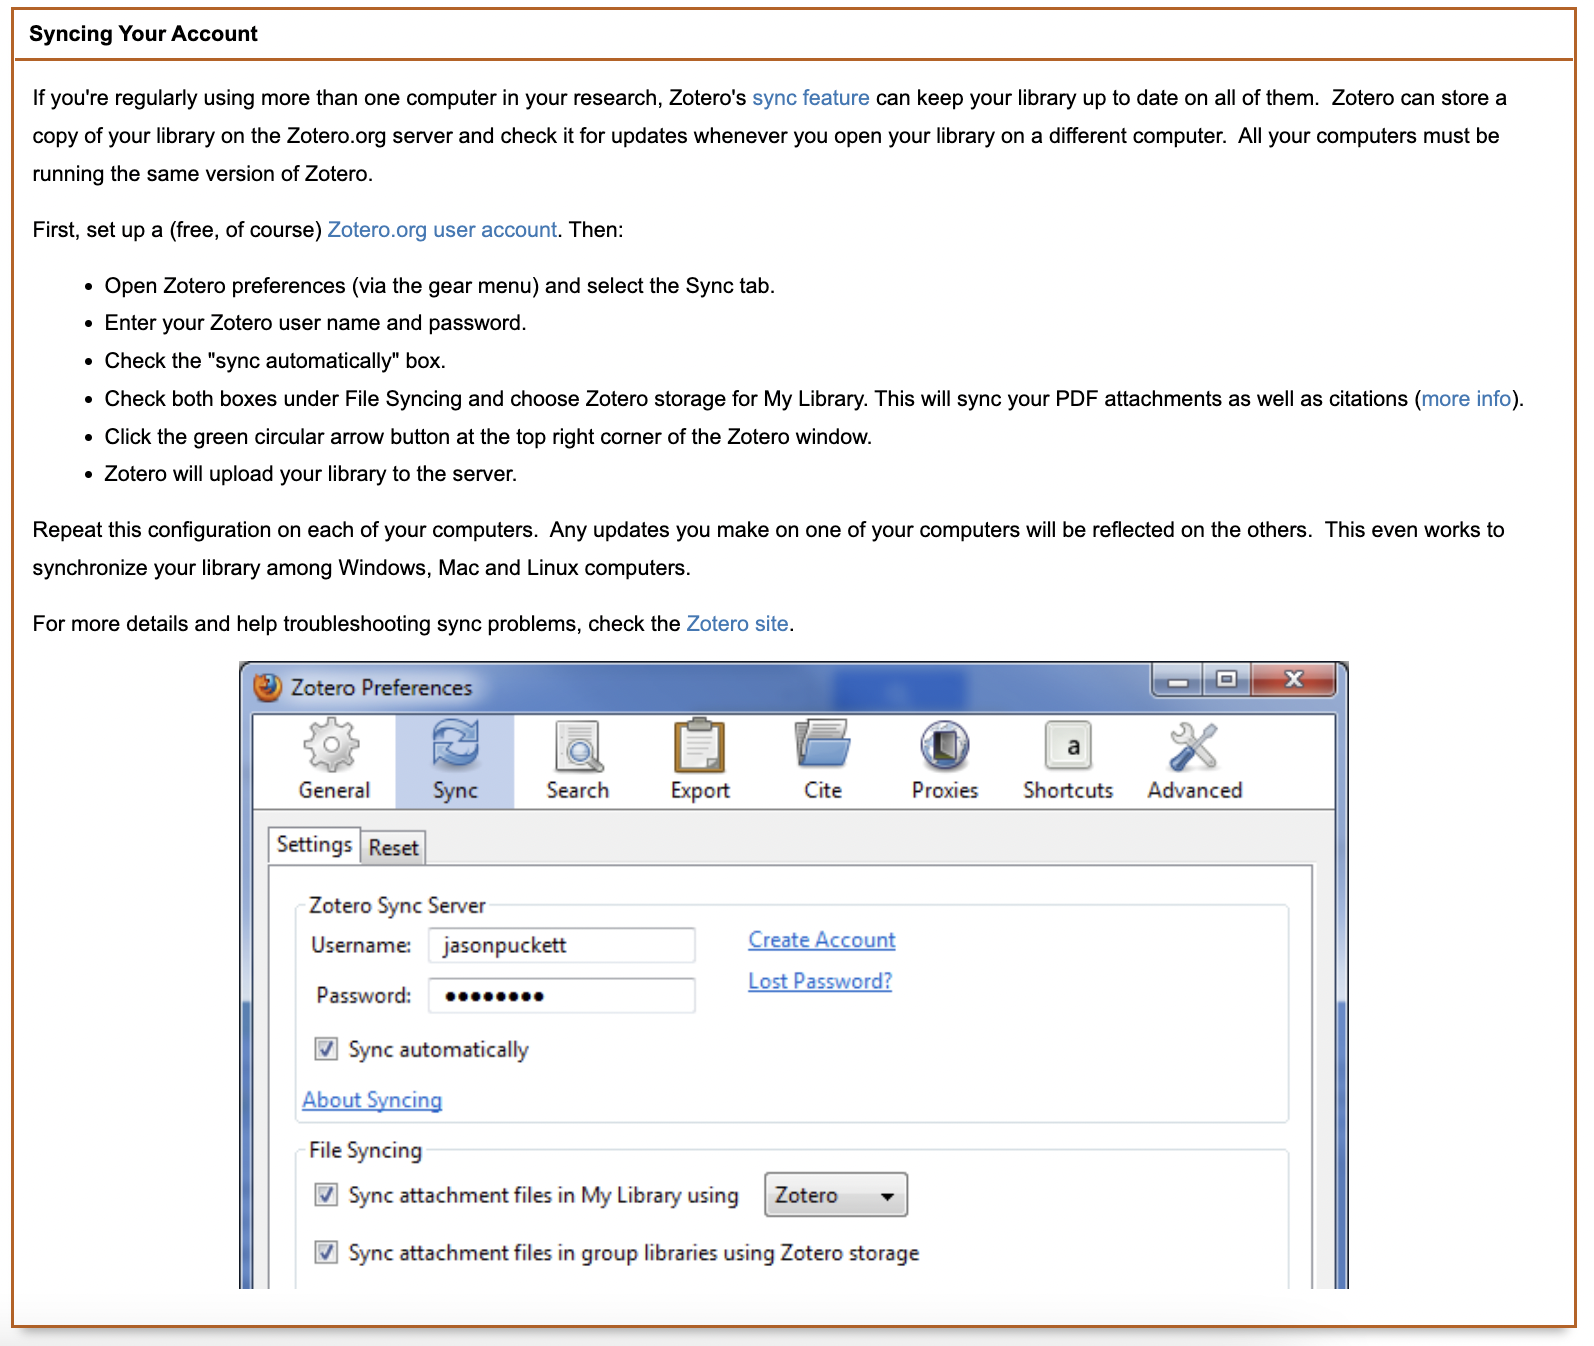
\includegraphics[width=22.14in]{images/zoterosyncing} \end{center}

To connect to the CCB Zotero Reference Group, navigate to \href{https://www.zotero.org/groups/4734848/ccbucr}{this link}. If you do not have access to the Group page, please send a request that you be added to the CCB PI.

For more information on how to use Zotero, check out these links:

\begin{itemize}
\tightlist
\item
  \href{https://guides.lib.ucr.edu/c.php?g=171064\&p=1126842}{UC Riverside Zotero Tips \& Tricks}
\item
  \href{https://www.zotero.org/support/quick_start_guide}{Zotero Quick Start Guide}
\item
  \href{https://www.zotero.org/support/groups}{Zotero Groups}
\item
  \href{https://www.youtube.com/watch?v=zuuOYjE8m98}{RStudio Citations} - add BibTex citation format in Zotero then quickly use .bib files in R to create references in markdown.
\end{itemize}

  \bibliography{book.bib,packages.bib}

\end{document}
